\chapter{Calculus of Communicating Systems}
Dati due processi $p_1$ ed $p_2$ si ha che essi sono specificati in \textbf{esecuzione concorrente} con l'utilizzo del simbolo $|$:
$$p_1 | p_2$$

L'esecuzione in concorrenza può portare a diverse complicanze qualora non venga rispettato, per esempio, un certo ordine di esecuzione. Si ha quindi il \textbf{non determinismo}, ovvero il risultato ottenuto dall'esecuzione dei programmi dipende dall'ordine di esecuzione di essi. Inoltre, si perde la composizionalità dei processi.
\begin{esempio}[\textbf{non determinismo e nessuna composizionalità}]
    Supponiamo di avere due programmi $p_1$ e $p_2$ definiti nel seguente modo: $$p_1 =\{x = V\} x = 2 \{x = 2\}$$ $$p_2 =\{x = V\} x = 3 \{x = 3\}$$ con $V$ che indica un qualunque valore.

    L'esecuzione in parallelo di questi due programmi mi permette di ottenere i seguenti risultati: $$ \{x = V\} \ p_1 | p_2 \ \{x = 2 \lor x = 3\}$$ avendo quindi una situazione di non determinismo. Inoltre, definendo un nuovo problema $p_1'$ possiamo osservare come la proprietà di composizionalità non risulta più valida. $$p_1' = \{x = V\} \ x = 1; x = x + 1 \ \{x = 2\}$$ Se proviamo a sostituire questo programma al posto di $p_1$ otteniamo: $$ \{x = V\} \ p_1' | p_2 \ \{x = 2 \lor x = 3 \lor x = 4\}$$
\end{esempio}

Hoare ha introdotto un nuovo paradigma di programmazione, il paradigma \textbf{CSP} (\textit{Communicating Sequential Processes}), il linguaggio macchina dei cosiddetti transputer. Non si ha più una memoria condivisa ma un insieme di processi ciascuno con una sua memoria privata. Si ha un'interazione tra processi tramite lo scambio di messaggi del tipo hand-shacking, avendo quindi la sincronizzazione, con lo scambio di informazioni. Viene fatto anche un processo particolare rappresentante la memoria condivisa. Avremo quindi: $$x \ | \ p_1 \ | \ p_2$$ dove $x$ che rappresenta la memoria condivisa dai due processi.

Milner propose infatti il lambda calcolo ($\lambda$-calcolo) per passare dal sequenziale al concorrente. Studia in modo approfondito la composizionalità, sfruttando la composizione tra funzioni, cercando di non perderla nel concorrente. Introduce quindi una sorta di $\lambda$-calcolo concorrente, introducendo il \textbf{CCS} (\textit{Calculus of Communicating Systems}), in cui pensa ad un calcolo algebrico per sistemi comunicanti. Adotta anche lui un paradigma che studia un sistema formato da componenti, chiamati processi. Questi processi comunicano tramite lo scambio sincrono di messaggi, con il modello hand-shacking.

Per la gestione di questo scambio di messaggi si utilizza la seguente notazione: 
\begin{itemize}
    \item \textbf{$a$}: indichiamo un processo generico che invia il messaggio.
    \item \textbf{$\overline{a}$}: indichiamo un processo generico che riceve.
\end{itemize}

Un sistema, quindi, è un insieme di processi il cui comportamento è gestito da un calcolo algebrico, si punta alle algebre di processi, ovvero linguaggi di specifica di sistemi concorrenti che si ispirano al calcolo dei sistemi comunicanti.

I messaggi di scambio corrispondono ad uno scambio di valori di variabili e questo è rappresentabile dall'algebra. I processi possono interagire anche con l'ambiente esterno. Dato un sistema $P$, si scrive: $$ P = p_1 \ | \ p_2 \ | \ p_3$$ se $P$ è formato dai processi $p_1$, $p_2$ e $p_3$, processi che sono interagenti a due a due. Ogni processo ha comunque una memoria privata.

Grazie alla comunicazione con l'ambiente esterno non si ha più un sistema chiuso.

Milner risolve il problema della composizionalità tramite l'uso di diverse porte che permettono ad un processo di comunicare con altri o con l'ambiente esterno. Quindi ogni processo può essere visto come un insieme di sotto-processi interagenti che però interagiscono tramite sincronizzazione con i processi esterni tramite una porta. Bisogna comunque mantenere il comportamento complessivo. Per il processo esterno è come se sostituissi il processo con cui comunica con il suo sotto-processo. Si introduce infatti l'\textbf{equivalenza all'osservazione}, che permette di sostituire un processo $p_i$ con uno $p_i'$ se sono equivalenti rispetto all'osservazione, ovvero se e solo se un qualsiasi osservatore esterno non è in grado di distinguere i due processi. 

Con il termine osservare ci si riferisce all’interazione con il sistema dove agisce il processo. Questo deve essere valido per ogni possibile osservatore. Se questo è garantito la sostituzione di un processo non va a modificare l'esecuzione complessiva, senza incorrere in deadlock o altre problematiche.

Vedremo quindi:
\begin{itemize}
    \item Il calcolo “puro” di sistemi comunicanti CCS, definendone la semantica attraverso \textbf{LTS} (\textit{Labeled Transition System}), rappresentando i processi come nodi e le azioni come archi etichettati.
    \item L'equivalenza all'osservazione e la bisimulazione.
\end{itemize}
\section{Labeled Transition System (LTS)}
I \textbf{Labeled Transition System} (LTS) sono molto usati per rappresentare sistemi concorrenti. Questo modello ha origine dal modello degli automi a stati finiti, i quali sono però usati come riconoscitori di linguaggi.

Negli LTS non si ha l'obbligo di avere un insieme finito di stati.
\begin{definizione}
    Possiamo definire un LTS come una quadrupla: $$LTS = (S, Act, T, s_0)$$ dove 
    \begin{itemize}
        \item \textbf{$S$}: rappresenta un insieme di stati.
        \item \textbf{$Act$}: è un insieme di nomi di azioni.
        \item \textbf{$T$}: è una relazione definita come: $$T \subseteq S \times Act \times S$$ tale che: $$\{(s, a, s') \ | \ s, s' \in S \ \land \ a \in Act \}$$ e può essere rappresentata come: $$s \xrightarrow{a} s'$$
        \item \textbf{$s_0$}: rappresenta lo stato iniziale. Questo campo non sempre è presente.
    \end{itemize}
\end{definizione}

La transizione $s \xrightarrow{a} s'$ può essere estesa a $w \in Act^{\ast}$ avendo più azioni se e solo se:
\begin{itemize}
    \item se $w = \varepsilon$ allora $s \equiv s'$
    \item se $w = a \cdot x$ con $a \in Act$ e $x \in Act^{\ast}$ se e solo se: $$s \xrightarrow{a} s'' \ \text{e} \ s'' \xrightarrow{x} s'$$
\end{itemize}

Ho che $s \rightarrow s'$ se e solo se $\exists a \in Act$  tale che $s \xrightarrow{a} s'$. Quindi ho: $$\rightarrow \ = \bigcup_{a \in Act} \xrightarrow{a}$$ Ho che $s \xrightarrow{\ast} s'$ se e solo se $\exists w \in Act^{\ast}$ tale che $s \xrightarrow{w} s'$. Si ha che: $$\xrightarrow{\ast} \ = \bigcup_{w \in Act^{\ast}} \xrightarrow{w}$$ $$\xrightarrow{\ast} \ \subseteq S \times S$$

La relazione $\xrightarrow{\ast}$ è la chiusura riflessiva e transitiva della relazione $\rightarrow$ tale relazione non è simmetrica, avendo sempre $s \xrightarrow{\ast} s$ ed essendo garantita la transitività.
\section{Calculus of Communicating Systems (CCS)}
\begin{definizione}
    Per definire il \textbf{Calculus of Communicating Systems} (CCS) "puro" dobbiamo definire:
    \begin{itemize}
        \item  $K$, ovvero un insieme di nomi di processi che possono anche essere simboli di un alfabeto.
        \item  $A$, ovvero un insieme di nomi di azioni, che sono o azioni di sincronizzazione con l'ambiente o le componenti del sistema.
        \item $\overline{A}$, ovvero l'insieme di nomi delle coazioni contenute in $A$, $\forall \ a \ \in A \ \exists \ \overline{a} \ \in \ \overline{A}$ quindi: $$\overline{A} = \{\overline{a} \ | \ a \ \in \ A\}$$ e ovviamente si ha nel: $$\overline{\overline{a}} = a$$ 
        \item $Act = A \ \cup  \ \overline{A} \ \cup \ \{\tau\}$ dove $\tau \notin A$ corrisponde all'azione di sincronizzazione tra $a$ e $\overline{a}$, ovvero la sincronizzazione è avvenuta. Le prime due sono azioni osservabili e si indica con: $$L = A \cup \overline{A}$$ mentre $\tau$ non è osservabile. Ricordando che osservare un'azione significa poter interagire con essa.
    \end{itemize}
\end{definizione}
\begin{definizione}
    I processi CCS sono di fatto operazioni CCS e un sistema CCS è definito da una collezione di processi $p \in K$ e si avranno: $$p = espressione \ CCS$$ e si avrà solo un'equazione $\forall p \in K$.
\end{definizione}
Definiamo meglio i processi CCS e, ad ogni processo, abbiniamo l'LTS, che sarà una struttura del tipo: $$(Proc_{CCS}, Act, T, p_0)$$ dove la transizione $T$ viene rappresentata con delle regole di inferenza strutturate nel seguente modo: $$\frac{Premesse}{Conseguenze}$$ Dare un significato tramite LTS, regole di inferenza e sintassi, è detto semantica operazionale strutturale.

Un processo CCS può essere:
\begin{itemize}
    \item \textbf{Nil} o 0 che ha un solo stato senza transazioni.
    \begin{figure}[!ht]
        \centering
        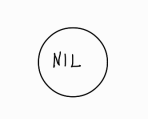
\includegraphics[scale=0.3]{img/ccs/nil.png}
        \caption{Rappresentazione grafica dell'operazione Nil}
    \end{figure}
    \item \textbf{Prefisso}: in cui si ha $\alpha \cdot P$ dove $P \in Proc_{CCS}$ e $\alpha \in Act$. Questo può essere rappresentato mediante inferenza nel seguente modo: $$\frac{}{\alpha \cdot P \xrightarrow{\alpha} P}$$
    \begin{figure}[!ht]
        \centering
        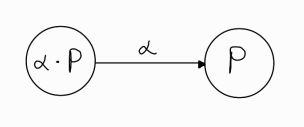
\includegraphics[scale=0.5]{img/ccs/prefisso.png}
        \caption{Rappresentazione grafica dell'operatore prefisso}
    \end{figure}
    \item \textbf{Somma}: siano $p_1, p_2 \in Proc_{CCS}$ posso comporli utilizzando l'operatore $+$ nel seguente modo $p_1 + p_2$. In questo caso per definire le regole di inferenza necessito $\alpha, \beta \in Act$ e $p_1', p_2' \in Proc_{CCS}$. $$\frac{p_1 + p_2 \xrightarrow{\alpha} p_1'}{p_1 + p_2 \xrightarrow{\alpha} p_1'}$$ oppure $$\frac{p_1 + p2 \xrightarrow{\beta} p_2'}{p_1 + p_2 \xrightarrow{\beta} p_2'}$$
    \begin{figure}[!ht]
        \centering
        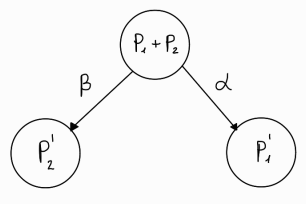
\includegraphics[scale=0.5]{img/ccs/somma.png}
        \caption{Rappresentazione grafica dell'operatore prefisso}
    \end{figure}
    Questo caso può essere generalizzato per più processi. Posso avere $\sum_{i \in I} p_i$ avendo multiple somme di processi: $$\frac{p_j \xrightarrow{\alpha} p_j'}{\sum_{i \in I} p_i \xrightarrow{\alpha} p_j'}, \ j \in J$$ Nel caso di $I = \emptyset$ avrò $\sum_{i \in I} p_i = Nil$

    Nell'applicazione di questa operazione possono presentarsi situazioni di non determinismo, ad esempio avendo $p_1 = \alpha \cdot p_1'$ e $p_2 = \alpha \cdot p_2'$.
    \item \textbf{Composizione parallela}: indicata con il simbolo $p_1 | p_2$ e utilizzando le regole di inferenza: $$\frac{p_1 \xrightarrow{\alpha} p_1'}{p_1 | p_2 \xrightarrow{\alpha} p_1' | p_2}$$ oppure $$\frac{p_2 \xrightarrow{\alpha} p_2'}{p_1 | p_2 \xrightarrow{\alpha} p_1 | p_2'}$$ oppure $$\frac{p_1 \xrightarrow{\alpha} p_1' \land p_2 \xrightarrow{\overline{\alpha}} p_2'}{p_1 | p_2 \xrightarrow{\tau} p_1' | p_2'}$$ in quest'ultimo caso, non potremo più avere altre sincronizzazioni.
    \begin{figure}[!ht]
        \centering
        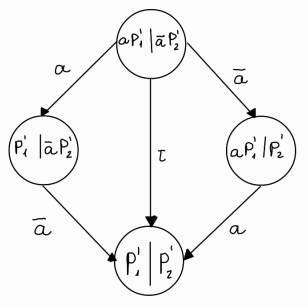
\includegraphics[scale=0.5]{img/ccs/parallela.png}
        \caption{Rappresentazione grafica dell'operatore prefisso}
    \end{figure}
    \item \textbf{Restrizione}: sia $L \subseteq A$. Si ha che: $$p_{\setminus L}$$ indica che il processo $p$ non può interagire con il suo ambiente con azioni in $L \cup \overline{L}$ ma le azioni in $L \cup \overline{L}$ sono locali a $p$. $$\frac{p \xrightarrow{\alpha} p'}{ p_{\setminus L} \xrightarrow{\alpha} p'_{\setminus L}}$$
    \item \textbf{Rietichettatura}: ovvero il cambiamento di nome ad una componente, ad una certa azione, per poter riusare tale nome. Ho quindi una funzione $f$ tale che:
    \begin{equation}
        f: Act \to Act
    \end{equation}
    inoltre, deve sempre essere garantito che:
    \begin{itemize}
        \item $f(\tau) = \tau$
        \item $f(\overline{a}) = \overline{f(a)}$
    \end{itemize}

    Ho quindi $p_{[f]}$ tale che: $$\frac{p \xrightarrow{\alpha} p'}{p_{[f]} \xrightarrow{f(a)} p_{[f]}'}$$
    \item $K = P$ con $K$ uguale al nome di processo e $P \in Proc_{CCS}$. $$\frac{P \xrightarrow{\alpha} P' \land K = P}{K \xrightarrow{\alpha} P'}$$  
\end{itemize}
Quindi dato un CCS posso associare un LTS per quanto riguarda la semantica. Si ha una precedenza degli operatori, da quello con più precedenza a quello con meno precedenza:
\begin{enumerate}
    \item Restrizione
    \item Rietichettatura
    \item Prefisso
    \item Composizione parallela
    \item Somma
\end{enumerate}
\begin{esempio} [\textbf{Priorità degli operatori}]
    Avendo: $$R + a \cdot p | b \cdot Q_{\setminus L}$$ sarebbe: $$R + ((a \cdot p) | b \cdot (Q_{\setminus L}))$$  
\end{esempio}
Nel caso di composizione parallela posso eseguire le due operazioni o in una sequenza o nell'altra. Ho quindi una simulazione sequenziale non deterministica del comportamento del sistema dato dalla composizione parallela.

Per poter dire che una certa implementazione soddisfa ($\models$) una certa specifica o se due implementazioni diverse soddisfano la stessa specifica ci serve una relazione di equivalenza tra processi CCS, ovvero una relazione del tipo $$R \subseteq Proc_{ccs} \times Proc_{ccs}$$ tale che sia:
\begin{itemize}
    \item Riflessiva.
    \item Simmetrica.
    \item Transitiva.
\end{itemize}
Bisognerà inoltre astrarre:
\begin{itemize}
    \item Gli stati e considerare le azioni $Act$
    \item Dalle sincronizzazioni interne, ovvero dalle $\tau$
    \item Rispetto al non determinismo
\end{itemize}
Milner poi asserisce che $R$ deve essere inoltre una \textbf{congruenza} rispetto agli operatori del CCS.
\begin{definizione}
    Una relazione di equivalenza $R$ è una \textbf{congruenza} se e solo se: $$\forall p, q \in Proc_{CCS} \land \forall c[\cdot] \ \text{contesto} \ CCS $$ avendo quindi un contesto, un’espressione CCS con qualcosa di mancante, CCS sostituibile con qualcosa, allora: $$ \text{se} \ p\ R\ q \ \text{allora si ha} \ c[p] \ R \ c[q]$$
\end{definizione}
Sia $LTS_1 = (Q_1, Act_1, T_1, q_{01})$ e $LTS_1 = (Q_2, Act_2, T_2, q_{02})$ posso affermare che $LTS_1$ è \textbf{isomorfo} a $LTS_2$ se e solo se: $\alpha: Q_1 \to Q_2$ e $\beta: Act_1 \to Act_2$ sono corrispondenze biunivoche. Se valgono le seguenti assunzioni:
\begin{itemize}
    \item $\alpha(q_{01}) = q_{02}$
    \item $(q_1, a, q_1') \in T_1$ allora $(\alpha(q_1), \beta(a), \alpha(q_1')) \in T_2$
\end{itemize}
\begin{teorema}
    Dati due processi $p_1$ e $p_2$ a cui assegniamo i due LTS $LTS_1$ e $LTS_2$. I due processi sono \textbf{equivalenti} se $LTS_1$ e $LTS_2$ sono isomorfi. 
\end{teorema}
Oltre all'isomorfismo, due processi sono equivalenti se i due LTS ammettono le stesse sequenze di operazioni, prendendo l'equivalenza forte tra automi a stati finiti. Questa è detta \textbf{equivalenza rispetto alle tracce}, ovvero due programmi sono equivalenti se implementano la stessa sequenza di istruzioni.
    
Preso $p \in Proc_{CCS}$ posso definire l'insieme delle tracce di $p$ come:
\begin{equation}
    tracce(p) = \{w \in Act^{\ast}\ |\ \exists p' \in Proc_{CCS} \ p \xrightarrow{w} p'\}
\end{equation}
Suppongo, per ora, di non considerare le sincronizzazioni (quindi senza $\tau$).
\begin{itemize}
    \item Se $w = \varepsilon$ allora $p =  p'$
    \item Se $w = x_1 \cdot x_2 \cdot \dots \cdot x_n$ con $x_i \in Act$ $\exists p_1', p_2', \dots, p_n' \in Proc_{CCS}$ tale che: $$p \xrightarrow{x_1} p_1' \xrightarrow{x_2} \dots \xrightarrow{x_n} p_n' = p'$$
\end{itemize}
\begin{teorema}
    Preso $p' \in Proc_{CCS}$ è \textbf{equivalente rispetto alle tracce} a $p''$, indicato come: $$p' \stackrel{T}{\sim}  p''$$ se e solo se:
    \begin{equation}
        tracce(p') = tracce(p'')
    \end{equation}
\end{teorema}
Lo studio delle tracce, quindi, non è più sufficiente nel caso di sistemi concorrenti. Si necessità quindi di una nozione più restrittiva.
\subsection{Bisimulazione forte}
Dato che le tracce non sono sufficienti nel caso di processi concorrenti, si definisce il concetto di \textbf{bisimulazione}. 
\begin{definizione}
    Data una relazione binaria $R \subseteq Proc_{CCS} \times Proc_{CCS}$ è una relazione di \textbf{bisimulazione} (\textbf{forte}) se e solo se: $$\forall p, q \in Proc_{CCS}: \ p R q$$ vale che: 
    \begin{itemize}
        \item $\forall \alpha \in Act = A \cup \overline{A} \cup \{\tau\}$ se ho $p \xrightarrow{\alpha} p'$ allora deve esistere un processo $$\exists q' \ \text{tale che} \ q \xrightarrow{\alpha} q' \ \text{e si ha} \ p'Rq'$$
        \item E viceversa, ovvero $\forall \alpha \in Act = A \cup \overline{A} \cup \{\tau\}$ se ho $q \xrightarrow{\alpha} q'$ allora deve esistere un processo $$\exists p' \ \text{tale che} \ p \xrightarrow{\alpha} p' \ \text{e si ha} \ p'Rq'$$
    \end{itemize}
    Due processi $p$ e $q$ sono fortemente bisimili, indicato con la notazione: $$p \stackrel{Bis}{\sim} q$$ se e solo se $\exists R \subseteq Proc_{CCS} \times Proc_{CCS}$, relazione di bisimulazione forte tale che: $$p R q$$ $$\stackrel{Bis}{\sim} = \bigcup \{R \subseteq Proc_{CCS} \times Proc_{CCS} \ | \ R \ \text{è una relazione di bisimulazione forte}\}$$
\end{definizione}
\begin{teorema}
    Se prendo $\stackrel{Bis}{\sim}  \subseteq Proc_{CCS} \times Proc_{CCS}$ si dimostra che è:
    \begin{itemize}
        \item Riflessiva.
        \item Simmetrica.
        \item Transitiva.
    \end{itemize}
    e quindi è una relazione di equivalenza. Quindi: $$p \stackrel{Bis}{\sim} q \Longleftrightarrow \forall \alpha \in Act \ \text{se} \ p \xrightarrow{\alpha} p'$$ allora $$\exists q' \ \text{tale che} \ q \xrightarrow{\alpha} q' \ \land \ p' \stackrel{Bis}{\sim} q'$$ e se: $$q \xrightarrow{\alpha} q'$$ allora $$\exists p' \ \text{tale che} \ p \xrightarrow{\alpha} p' \ \land \ p' \stackrel{Bis}{\sim} q'$$ 
\end{teorema}
\begin{teorema}
    Se due processi sono fortemente bisimili allora sono sicuramente equivalenti rispetto alle tracce. Non vale il viceversa.
\end{teorema}
Per vedere che due processi sono bisimili devo quindi, per ogni esecuzione, ottenere due processi ancora bisimili (potendo quindi fare le azioni corrispondenti da entrambe le parti).
\begin{esempio}
    Consideriamo i processi $p_1 = a \cdot b \cdot Nil + a \cdot c \cdot Nil$ e $p_2 = a \cdot (b \cdot Nil + c \cdot Nil)$
    \begin{figure}[!ht]
        \centering
        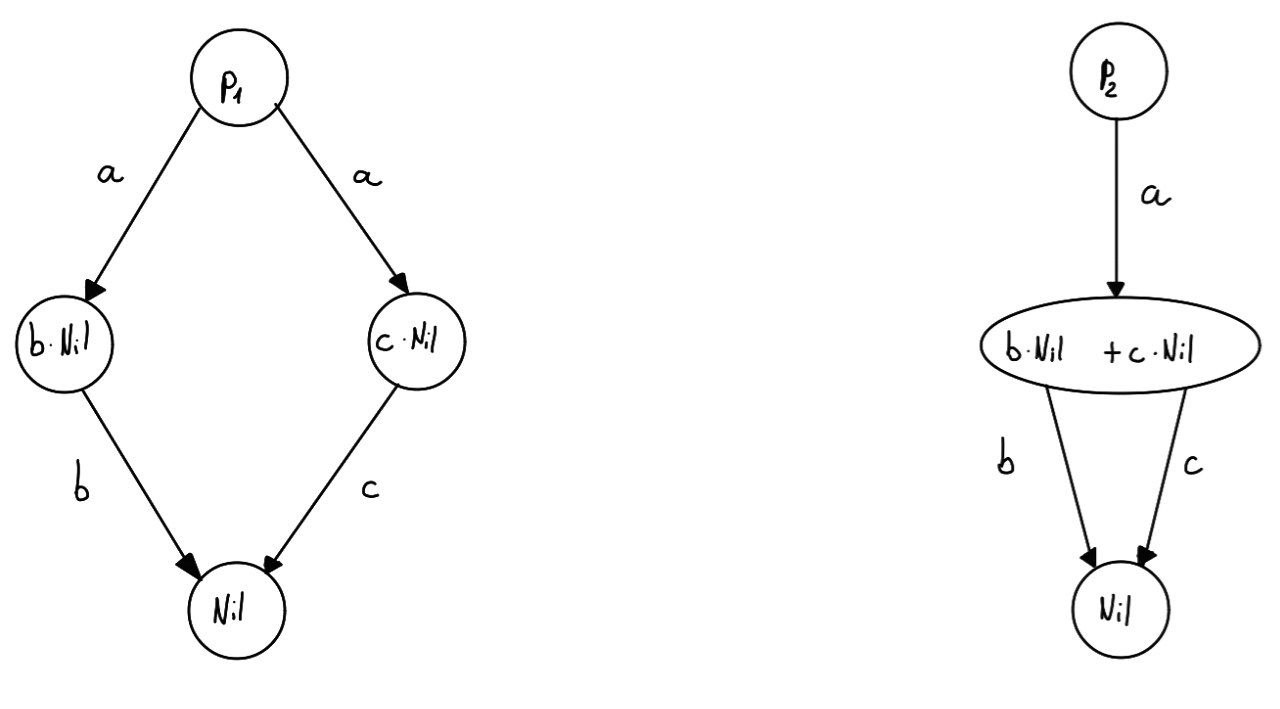
\includegraphics[scale=0.25]{img/ccs/Esempio1.png}
        \caption{LTS dei processi $p_1$ e $p_2$}
    \end{figure}
    
    Osserviamo subito che i due processi sono equivalenti rispetto alle tracce, difatti:
    \begin{itemize}
        \item $Tracce(p_1) = \{\varepsilon, a, a \cdot b, a \cdot c\}$
        \item $Tracce(p_2) = \{\varepsilon, a, a \cdot b, a \cdot c\}$
    \end{itemize}

    Vediamo se i due processi sono anche bisimili.
    \begin{itemize}
        \item Da $p_1$ possiamo eseguire l'azione $a$ e possiamo fare lo stesso anche da $p_2$. Dobbiamo però chiederci se gli stati di arrivo sono anche essi in relazione di bisimulazione.
        \item Gli stati interessati sono $b \cdot Nil$ e $b \cdot Nil + c \cdot Nil$: dal primo possiamo eseguire $b$, che è fattibile anche dal secondo, ma dal secondo possiamo eseguire $c$, che non è eseguibile dal primo (la bisimulazione richiede che entrambi gli stati siano simili tra loro), dunque i due processi non sono bisimili.
    \end{itemize}
    Formalmente:
    \begin{itemize}
        \item $p_1 \xrightarrow{a} b \cdot Nil$
        \item $p_2 \xrightarrow{a} b \cdot Nil + c \cdot Nil$
    \end{itemize}
    $b \cdot Nil \stackrel{Bis}{\not\sim} b \cdot Nil + c \cdot Nil$ inoltre, possiamo osservare che: $b \cdot Nil \stackrel{T}{\not\sim} b \cdot Nil + c \cdot Nil$ 
\end{esempio}
\begin{esempio}
    Consideriamo due processi che simulano dei buffer che possono contenere due elementi:
    \begin{itemize}
        \item $B_0^1 | B_0^1$ dove $B_0^1 = in \cdot B_1^1$ e $B_1^1 = \overline{out} \cdot B_0^1$
        \item $B_0^2 = in \cdot B_1^2$, $B_1^2= \overline{out} \cdot B_0^2 + in \cdot B_2^2$ e $B_2^2 = \overline{out} \cdot B_1^2$
    \end{itemize}

    \begin{figure}[!ht]
        \centering
        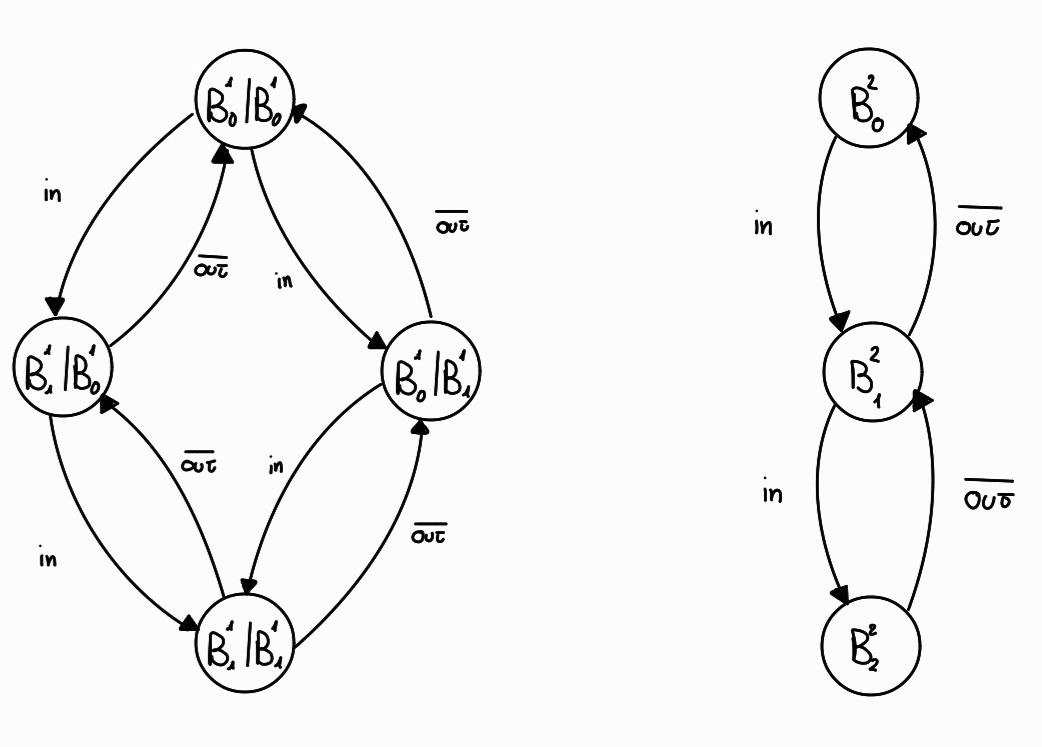
\includegraphics[scale=0.25]{img/ccs/Esempio 2.png}
        \caption{LTS dei processi $B_0^1 | B_0^1$ e $B_0^2$}
    \end{figure}

    In questo esempio, possiamo osservare che: $$(B_0^1 | B_0^1) \stackrel{Bis}{\sim} B_0^2$$ $B_0^2$ può essere messo in relazione con $B_0^1| B_0^1$ in quanto se vado in uno tra $B_1^1 | B_0^1$ e $B_0^1 | B_1^1$ posso sempre fare $in$ e $\overline{out}$. Inoltre, Posso fare un discorso analogo per $B_2^2$ e $B_1^1 | B_1^1$. Essendo questi ultimi quindi bisimili lo sono anche il nodo centrale coi due possibili nodi nel caso della composizione e di conseguenza lo sono anche $B_0^2$ e $B_0^1 | B_0^1$.
\end{esempio}

Cerco quindi di astrarre dalle interazioni interne ($\tau$), introducendo l'equivalenza debole, volendo astrarre rispetto alle azioni $\tau$ , introducendo il concetto di bisimulazione debole.

Vediamo quindi le proprietà della bisimulazione forte:
\begin{itemize}
    \item La bisimulazione forte è una congruenza rispetto agli operatori del CCS. Quindi se ho $p \stackrel{Bis}{\sim} q$ con $p, q \in Proc_{CCS}$ vale: $$\alpha \cdot p \stackrel{Bis}{\sim}  \alpha \cdot q \ \forall \ \alpha \in Act$$
    \item Vale la proprietà commutativa rispetto alla composizione $+$: $$p + r \stackrel{Bis}{\sim} q + r \ \land \ r + p \stackrel{Bis}{\sim} r + q, \ \ \forall r \in Proc_{CCS}$$
    \item Vale la proprietà commutativa rispetto alla composizione $|$: $$p | r \stackrel{Bis}{\sim} q | r \ \land \ r | p \stackrel{Bis}{\sim} r | q, \ \ \forall r \in Proc_{CCS}$$
    \item Per ogni funzione di rietichettatura $f : Act \to Act$ vale: $$p_{[f]} \stackrel{Bis}{\sim} q_{[f]}$$
    \item $p_{\backslash L} \stackrel{Bis}{\sim} q_{\backslash L}$
\end{itemize}

A queste proprietà possiamo aggiungere delle \textit{leggi} legate al fatto che gli operatori hanno delle proprietà. Dati $p, q, r \in Proc_{CCS}$ valgono le seguenti proprietà:
\begin{itemize}
    \item \textbf{Commutatività}: $$p + q \stackrel{Bis}{\sim} q + p \ \land \ p | q \stackrel{Bis}{\sim} q | p$$
    \item \textbf{Distributività}: $$(p + q) + r \stackrel{Bis}{\sim} p + (q + r) \ \land \ (p | q) | r \stackrel{Bis}{\sim} p | (q | r)$$
    \item \textbf{Leggi di assorbimento}: $$p + Nil \stackrel{Bis}{\sim} p \ \land \ p | Nil \stackrel{Bis}{\sim} p$$
\end{itemize}
\subsection{Bisimulazione debole}
La bisimulazione forte rischia di essere troppo restrittiva. Si passa quindi alla definizione di \textbf{equivalenza debole rispetto alle tracce}: $$\stackrel{T}{\approx}$$ e \textbf{bisimulazione debole}: $$\stackrel{Bis}{\approx}$$
La definizione di queste nuove relazioni mi obbliga a modificare la definizione della funzione di transizione. La relazione di transizione debole è definita come: $$\Rightarrow \subseteq Proc_{CCS} \times Act \times Proc_{CCS}$$ Possiamo rappresentare tale funzione come: $$p \stackrel{\alpha}{\Rightarrow} p'$$ dove $\alpha \in Act$ se e solo se:
\begin{itemize}
    \item Se $\alpha = \tau$ allora posso eseguire una sequenza qualsiasi, anche nulla, di $\tau$: $$p \xrightarrow{\tau}^{\ast} p'\begin{cases}
        p = p' & \text{se non ci sono } \tau \text{ da eseguire} \\
        p \xrightarrow{\tau} p_1 \xrightarrow{\tau} \dots \xrightarrow{\tau} p' & \text{altrimenti}
    \end{cases}$$
    \item Se $\alpha \in A \cup \overline{A}$ allora vale: $$p \xrightarrow{\tau}^{\ast} \xrightarrow{\alpha} \xrightarrow{\tau}^{\ast}$$
\end{itemize}
Come fatto per la relazione forte, definiamo la relazione di transizione per sequenze di azioni $w \in Act^{\ast}$: $$p \stackrel{w}{\Rightarrow} p'$$ se e solo se:
\begin{itemize}
    \item Se $w = \varepsilon$ oppure $w = \tau^{\ast}$ allora ho: $$p \xrightarrow{\tau}^{\ast} p'$$
    \item Se $w = a_1\dots a_n$ con $a_i \in A \cup \overline{A}$ allora: $$p \stackrel{a_1}{\Rightarrow} p_1 \stackrel{a_2}{\Rightarrow} \dots \stackrel{a_n}{\Rightarrow} p'$$ dove ogni $a_i$ può essere preceduto/seguito da una qualsiasi sequenza di $\tau$.
\end{itemize}
\begin{definizione}
    Definiamo l'\textbf{equivalenza debole rispetto alle tracce}, la quale è rappresentata come: $$p \stackrel{T}{\approx} q$$ se e solo se: $$Tracce_{\Rightarrow} (p) = Tracce_{\Rightarrow}(q)$$ ovvero: $$\forall w \in (A \cup \overline{A}) \ \text{ho che} \ p \stackrel{w}{\Rightarrow} \iff q \stackrel{w}{\Rightarrow}$$ ovvero se i due processi possono eseguire la stessa sequenza di azioni.
\end{definizione}
Posso definire le tracce come: $$Tracce_{\Rightarrow}(p) = \{w \in (A \cup \overline{A})^{\ast} | p \stackrel{w}{\Rightarrow}\}$$
\begin{definizione}
    Data una relazione $R$ definita come: $$R \subseteq Proc_{CCS} \times Proc_{CCS}$$ Dico che $R$ è una relazione di \textbf{bisimulazione debole} se e solo se: $$\forall p, q \in Proc_{CCS} \ \text{tale che } p R q \ \text{vale che } \forall a \in Act$$
    \begin{itemize}
        \item Se $p \xrightarrow{a} p'$ allora $\exists q'$ tale che $q \stackrel{a}{\Rightarrow} q'$ e $p'Rq'$
        \item E deve valere anche il viceversa: $q \xrightarrow{a} q'$ allora $\exists p'$ tale che $p \stackrel{a}{\Rightarrow} p'$ e $p'Rq'$
    \end{itemize}
\end{definizione}
Due processi $p$ e $q$ sono in relazione di bisimulazione debole: $$p \stackrel{Bis}{\approx} q$$ se e solo se esiste una relazione di bisimulazione $R$ tale che: $$p R q$$ si ha che vale $$\stackrel{Bis}{\approx} = \bigcup \{R | R \ \text{è di bisimulazione debole}\}$$
\begin{esempio}
     Consideriamo i processi $r = a \cdot (b \cdot Nil + \tau \cdot c \cdot Nil)$ e $k = a \cdot (b \cdot Nil + \tau \cdot c \cdot Nil) + a \cdot c \cdot Nil$.
    \begin{figure}[!ht]
        \centering
        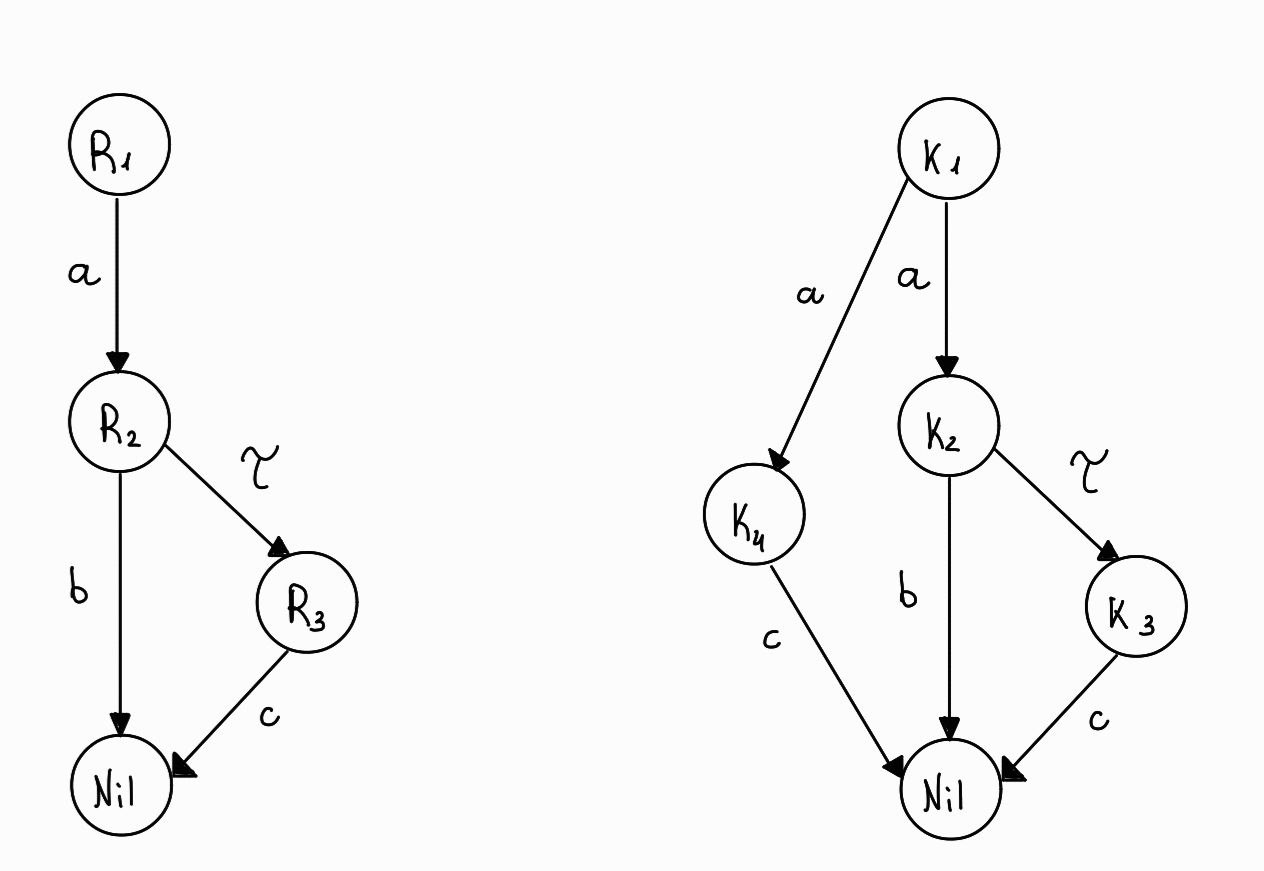
\includegraphics[scale=0.25]{img/ccs/Esempio3.png}
        \caption{LTS di $r$ e $k$}
    \end{figure}
    $$r \stackrel{Bis}{\approx} k$$
\end{esempio}
\newpage
\subsubsection{Gioco verifica bisimulazione debole}
Per confrontare due processi $p$ e $q$ si può utilizzare un gioco $G(p, q)$ con 2 giocatori:
\begin{itemize}
    \item \textbf{Attaccante}: il quale cerca di dimostrare che $p \stackrel{Bis}{\not\approx} q$
    \item \textbf{Difensore}: il quale cerca di dimostrare che $p \stackrel{Bis}{\approx} q$
\end{itemize}
Un gioco è composto da più partite, dove ogni partita è una sequenza finita o infinita di configurazioni: $$(p_0, q_0), (p_1, q_1), \dots, (p_i, q_i), \dots$$ In ogni mano si passa dalla configurazione corrente $(p_i, q_i)$ alla successiva $(p_{i + 1}, q_{i + 1})$ con le seguenti regole:
\begin{itemize}
    \item L'Attaccante sceglie uno dei due processi della configurazione corrente $(p_i, q_i)$ e fa una $\xrightarrow{\alpha}$ mossa $(\alpha \in Act)$
    \item Il Difensore deve rispondere con una $\stackrel{\alpha}{\Rightarrow}$ mossa nell'altro processo.
\end{itemize}
La coppia di processi $(p_{i+1}, q_{i+1})$ così ottenuta diventa la nuova configurazione corrente. La partita continua con un'altra mano.

La partita può terminare in uno dei due seguenti modi:
\begin{itemize}
    \item Se un giocatore non può muovere, l'altro vince.
    \item Se la partita è infinita, vince il difensore.
\end{itemize}
Diverse partite possono concludersi con vincitori diversi, ma per ogni gioco, un solo giocatore può vincere ogni partita.

Una \textbf{strategia} per un giocatore è un insieme di regole che indicano di volta in volta che mossa fare. Tali regole dipendono solo dalla configurazione corrente. Un giocatore ha una \textbf{strategia vincente} per un gioco $G(p, q)$ se seguendo quella strategia è in grado di vincere tutte le partite del gioco.
\begin{teorema}
    Per ogni gioco $G(p, q)$, solo uno dei due giocatori ha una strategia vincente.
\end{teorema}
\begin{teorema}
    \begin{itemize}
        \item L'Attaccante ha una strategia vincente per $G(p, q)$ se e solo se $p \stackrel{Bis}{\not\approx} q$.
        \item Il Difensore ha una strategia vincente per $G(p, q)$ se e solo se  $p \stackrel{Bis}{\approx} q$.
    \end{itemize}
\end{teorema}
\begin{nota}
    Il gioco della bisimulazione può essere usato sia per dimostrare che due processi sono bisimili, che per dimostrare che non lo sono.
\end{nota}
Per dimostrare che i processi sono Bisimili, bisogna mostrare che il Difensore ha una strategia vincente, cioè che, per ogni mossa dell'Attaccante, il Difensore ha almeno una mossa che lo porterà a vincere.

Per dimostrare che i processi non sono Bisimili, bisogna mostrare che l'Attaccante ha una strategia vincente, cioè che, in ogni configurazione, l'Attaccante è in grado di scegliere su quale processo operare e con quale azione, in modo che per ogni successiva mossa del Difensore, l'Attaccante ha almeno una mossa che lo porterà a vincere.
\section{Proprietà}
Siano $p, q \in Proc_{CCS}$:
\begin{itemize}
    \item Se $LTS(p)$ è isomorfo a $LTS(q)$ allora $p \simeq q$.
    \item Deve astrarre dagli stati.
    \item Se $p \simeq q$ allora le tracce di $p$ e $q$ sono equivalenti: $$Tracce(p) = Tracce(q)$$
    \item Se $p \simeq q$ allora $p$ e $q$ devono avere la stessa possibilità di generare deadlock nell'interazione con l'ambiente.
    \item $\simeq$ deve essere una congruenza rispetto agli operatori CCS: deve essere possibile sostituire un sotto-processo con un suo equivalente senza modificare il comportamento complessivo del sistema.
\end{itemize}
Siano $p, q \in Proc_{CCS}$ l'equivalenza rispetto alle tracce forte gode delle seguenti proprietà:
\begin{itemize}
    \item Se $LTS(p)$ è isomorfo a $LTS(q)$ allora $p \stackrel{T}{\sim} q$.
    \item Astrae dagli stati.
    \item Se $p \stackrel{T}{\sim} q$ se e solo se le tracce di $p$ e $q$ sono equivalenti: $$Tracce(p) = Tracce(q)$$
    \item $\stackrel{T}{\sim}$ è una congruenza rispetto agli operatori CCS.
    \item Non garantisce di preservare il deadlock o l'assenza di deadlock, nell'interazione con l'ambiente.
\end{itemize}
Siano $p, q \in Proc_{CCS}$ la bisimulazione forte gode delle seguenti proprietà:
\begin{itemize}
    \item Se $LTS(p)$ è isomorfo a $LTS(q)$ allora $p \stackrel{Bis}{\sim} q$.
    \item Astrae dagli stati.
    \item Se $p \stackrel{Bis}{\sim} q$ se le tracce di $p$ e $q$ sono equivalenti: $$Tracce(p) = Tracce(q)$$
    \item $\stackrel{Bis}{\sim}$ è una congruenza rispetto agli operatori CCS.
    \item Preservare il deadlock o l'assenza di deadlock, nell'interazione con l'ambiente.
\end{itemize}
L'equivalenza rispetto alle Tracce forte è più restrittiva dell'equivalenza rispetto alle Tracce debole. Siano $p, q \in Proc_{CCS}$ l'equivalenza rispetto alle tracce debole gode delle seguenti proprietà:
\begin{itemize}
    \item Se $LTS(p)$ è isomorfo a $LTS(q)$ allora $p \stackrel{T}{\approx} q$.
    \item Astrae dagli stati.
    \item Se $p \stackrel{T}{\approx} q$ se e solo se le tracce di $p$ e $q$ sono equivalenti: $$Tracce(p) = Tracce(q)$$
    \item $\stackrel{T}{\approx}$ è una congruenza rispetto agli operatori CCS.
    \item Non garantisce di preservare il deadlock o l'assenza di deadlock, nell'interazione con l'ambiente.
\end{itemize}
La bisimulazione forte è più restrittiva della bisimulazione debole: $$p \stackrel{Bis}{\sim} q \Rightarrow p \stackrel{Bis}{\approx} q \ ( \stackrel{Bis}{\sim} \subseteq \stackrel{Bis}{\approx})$$ La bisimulazione forte (debole) è più restrittiva dell'equivalenza rispetto alle Tracce forte (debole) $$p \stackrel{Bis}{\sim} q \Rightarrow p \stackrel{T}{\sim} q \ e \ p \stackrel{Bis}{\approx} q \Rightarrow p \stackrel{T}{\approx} q$$ $$(\stackrel{Bis}{\sim} \subseteq \stackrel{T}{\sim}) \ e \ (\stackrel{Bis}{\approx} \subseteq \stackrel{T}{\approx})$$
\begin{definizione}
    $p \in Proc_{CCS}$ è un processo deterministico se e solo se vale che: $$\forall x \in Act = A \cup \overline{A} \cup \{\tau\}, \ \text{se} \ p \xrightarrow{\ast} p' \ \text{e} \ p \xrightarrow{\ast} p'' \ \text{allora} \ p' = p''$$
\end{definizione}
Siano $p, q \in Proc_{CCS}$ se $p$ e $q$ sono deterministici e $p \stackrel{T}{\sim} q$ ($p \stackrel{T}{\approx} q$) allora $p \stackrel{Bis}{\sim} q$ ($p \stackrel{Bis}{\approx} q$).

Siano $p, q \in Proc_{CCS}$ la bisimulazione debole gode delle seguenti proprietà:
\begin{itemize}
    \item È un'equivalenza, la più grande relazione di Bisimulazione debole.
    \item Astrae da azioni non osservabili ($\tau$) e dai cicli inosservabili ($\tau \ loop$).
    \item Preservare il deadlock o l'assenza di deadlock, nell'interazione con l'ambiente.
\end{itemize}
\begin{teorema}
    Se $p, q \in Proc_{CCS}$ tale che $p \stackrel{Bis}{\approx} q$, allora:
    \begin{itemize}
        \item $\alpha \cdot p \stackrel{Bis}{\approx} \alpha \cdot q \ \ \ \forall \alpha \in A_{CCS} = A \cup \overline{A} \cup \tau$
        \item $p | r \stackrel{Bis}{\approx} q | r \ \land \ r | p \stackrel{Bis}{\approx} r | q$ $\forall r \in Proc_{CCS}$
        \item $p_{[f]} \stackrel{Bis}{\approx} q_{[f]}$ $\forall f$ funzione di etichettatura.
        \item $p_{\backslash L} \stackrel{Bis}{\approx} q_{\backslash L}$ $\forall L \subseteq A$
    \end{itemize}
    La Bisimulazione debole è una congruenza rispetto agli operatori del CCS diversi da $+$ e ricorsione.

    Posso quindi affermare che la Bisimulazione debole non è una congruenza per il CCS.
\end{teorema}
\section{Congruenza}
Si definisce quindi, tramite assiomi, la più grande relazione di congruenza $\stackrel{C}{\approx}$ (per il CCS puro e senza ricorsione, con agenti finiti) che è contenuta nella relazione di Bisimulazione $\stackrel{Bis}{\approx}$. $$\stackrel{C}{\approx} \subseteq \stackrel{Bis}{\approx} \subseteq Proc_{CCS} \times Proc_{CCS}$$ insieme finito di Assiomi $Ax$:
\begin{itemize}
    \item Ax \textit{corretto} ($Ax \vdash p = q \Rightarrow p \stackrel{C}{\approx} q$)
    \item Ax \textit{completo} ($p \stackrel{C}{\approx} q \Rightarrow Ax \vdash p = q$)
\end{itemize}
\begin{enumerate}
    \item $p + (q + r) \stackrel{C}{\approx} (p + q) + r$ e $p | (q | r) \stackrel{C}{\approx} (p | q) | r$
    \item $p + q \stackrel{C}{\approx} q + p$ e $p | q \stackrel{C}{\approx} q | p$
    \item $p + p \stackrel{C}{\approx} p$ (ma $p | p \stackrel{C}{\not\approx} p$)
    \item $p + Nil \stackrel{C}{\approx} p$ e $p | Nil \stackrel{C}{\approx} p$
    \item $p + \tau \cdot p \stackrel{C}{\approx} \tau \cdot p$
    \item $\mu \cdot \tau p \stackrel{C}{\approx} \mu \cdot p$
    \item $\mu \cdot (p + \tau \cdot q) \stackrel{C}{\approx} \mu \cdot (p + \tau \cdot q) + \mu \cdot q$
    \item Se $p$ e $q$ sono delle somme: $p = \sum_{i} \alpha_i \cdot p_i$ e $q = \sum_{j} \beta_j \cdot q_j$,  $\alpha, \beta \in Act$: $$p | q \stackrel{C}{\approx} \sum_{i} \alpha_i (p_{i} | q) + \sum_{j} \beta_{j} \cdot (p|q_{j}) + \sum_{\alpha_i = \overline{\beta}_{j}} \tau \cdot (p_{i} | q_{j})$$ (teorema di espansione di R. Milner) Questo assioma mi permette di rappresentare la composizione parallela come la somma di tutte le possibili alternative che si hanno con l'operazione di composizione parallela.
    \item $p[f] \stackrel{C}{\approx} \sum_{i} f(\alpha_i) \cdot (p_{i} [f])$ $\forall f$ funzione di etichettatura.
    \item $p_{\backslash L} \stackrel{C}{\approx} \sum_{\alpha_i,\overline{\alpha}_i \not\in L} \alpha_i \cdot (pi_{\backslash L})$ $\forall L \subseteq A$
\end{enumerate}